\paragraph{Example 1}{
\begin{lstlisting}[language=Python]
from BNumMet.Interpolation import pchip
x = list(np.arange(1, 7, 1))
y = [16, 18, 21, 17, 15, 12]
u = np.arange(0.8, 6.2, 0.05)
v = pchip(x, y, u)
# Plotting using Matplotlib
plt.plot(u, v, "b-", label="Interpolated")
plt.plot(x, y, "ro", label="Original Points")
plt.legend()
plt.title("PCHIP Interpolation")
plt.xlabel("x")
plt.ylabel("y")
plt.show()
\end{lstlisting}

\begin{figure}[H]
    \centering
    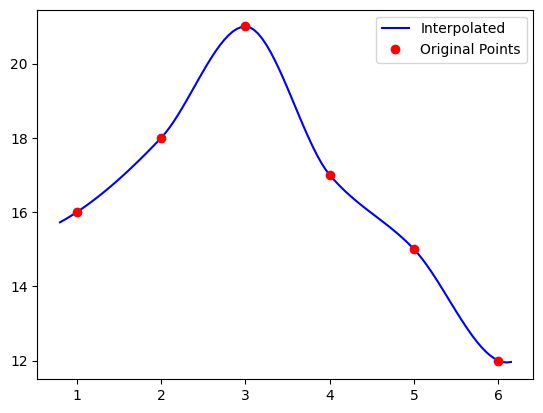
\includegraphics{Include/Images/Thesis/Documentation/Interpolation/PCHIP Example 1.png}
    \caption{PCHIP Example 1}
    \label{fig:PCHIP Example 1}
\end{figure}
}